                                                                                                              
%\pdfoutput=1
%\documentclass[fms,times]{cuparticle}
\documentclass[a4paper,11pt,twoside]{amsart}
\usepackage{amsmath}
\usepackage{geometry}
%\newproof{proof}{Proof}
\usepackage{amssymb, latexsym}
\usepackage{verbatim}
%\usepackage{amscd}
\usepackage{enumerate}
\usepackage{comment}
\usepackage{txfonts}
%\usepackage[breaklinks=true,hidelinks]{hyperref}

%\usepackage{psfig}
%\usepackage{graphicx}
%\usepackage{showkeys}  
%\usepackage{siunitx}
%\usepackage{tikz-cd}
%\usepackage{color}
%\usetikzlibrary{arrows}
% uncomment this when editing cross-references
%\numberwithin{equation}{section}
%\usepackage{hyperref}

%\volume{}
%\doi{}


% \usepackage{mathabx}


\usepackage{mathtools}%                  http://www.ctan.org/pkg/mathtools
\usepackage[tableposition=top]{caption}% http://www.ctan.org/pkg/caption
\usepackage{booktabs,dcolumn}%           http://www.ctan.org/pkg/dcolumn + http://www.ctan.org/pkg/booktabs

     
%\theoremstyle{plain}

\newtheorem{theorem}{Theorem}[section]
%\newtheorem{theorem}[theorem]{Theorem}
\newtheorem{proposition}[theorem]{Proposition}
\newtheorem{hypothesis}[theorem]{Hypothesis}
\newtheorem{lemma}[theorem]{Lemma}
\newtheorem{corollary}[theorem]{Corollary}
\newtheorem{conjecture}[theorem]{Conjecture}
\newtheorem{principle}[theorem]{Principle}
\newtheorem{claim}[theorem]{Claim}

%\theoremstyle{definition}

%\newtheorem{roughdef}[subsection]{Rough Definition}
\newtheorem{definition}[theorem]{Definition}
\newtheorem{remark}[theorem]{Remark}
\newtheorem{remarks}[theorem]{Remarks}
\newtheorem{example}[theorem]{Example}
\newtheorem{examples}[theorem]{Examples}
%\newtheorem{problem}[subsection]{Problem}
%\newtheorem{question}[subsection]{Question}

\newcommand\F{\mathbb{F}}
\newcommand\E{\mathbb{E}}
\newcommand\R{\mathbb{R}}
\newcommand\Z{\mathbb{Z}}
\newcommand\N{\mathbb{N}}
\newcommand\D{\mathbb{D}}
\newcommand\C{\mathbb{C}}
\newcommand\Q{\mathbb{Q}}
\newcommand\T{\mathbb{T}}
\renewcommand\Re{{\operatorname{Re\,}}}
\renewcommand\Im{{\operatorname{Im\,}}}
\newcommand\Log{{\operatorname{Log}}}
\newcommand\eps{\varepsilon}



\renewcommand\P{\mathbf{P}}


%%%%%%%%%%%%%%%%%%%%%%%%%%%%%%%%


\newcommand{\alert}[1]{{\bf \color{red} TODO: #1}}


\setlength\evensidemargin\oddsidemargin
%\setlength{\parindent}{0cm}

\begin{document}
\title[Zeroes of heat flow of Riemann $\xi$]{Zeroes of the heat flow evolution of the Riemann $\xi$ function at negative times: numerical experiments and heuristic justifications}

\author{D.H.J. Polymath}
\address{\tt{http://michaelnielsen.org/polymath1/index.php}}


\begin{abstract}
For each $t \in \R$, define the entire function
$$ H_t(z) \coloneqq \int_0^\infty e^{tu^2} \Phi(u) \cos(zu)\ du$$
where $\Phi$ is the super-exponentially decaying function
$$ \Phi(u) \coloneqq \sum_{n=1}^\infty (2\pi^2  n^4 e^{9u} - 3\pi n^2 e^{5u} ) \exp(-\pi n^2 e^{4u} ).$$
This is essentially the heat flow evolution of the Riemann $\xi$ function, introduced by de Bruijn.  The Riemann hypothesis asserts that the zeroes of $H_0$ are all real; recently, it was shown by Rodgers and Tao that the zeroes are no longer all real for $t<0$.

In this paper we investigate, through a combination of numerical experiments and heuristic asymptotics, the behavior of the zeroes of $H_t$ for negative times $t$.  The numerical experiments uncovered several striking patterns in the zeroes, for which we now also have heuristic justifications.  Firstly, there are complex zeroes $H_t(x+iy)$ clustered around the curves 
$$ y = |t| \log \frac{N}{\sqrt{n(n+1)}} - 1$$
for natural numbers $n$, where $N \coloneqq \sqrt{\frac{x}{4\pi} + \frac{t}{16}}$.  Secondly, for large values of the quantity 
$$ v := \frac{t^2}{64 \pi^2 N^3},$$
the only surviving real zeroes $H_t(x+iy)$ occur when $N$ is close to a half-integer, while for medium-sized values of $v$, the zeroes take on a ``sharkfin pattern'' that can be described asymptotically in terms of the zeroes of the Airy function.
\end{abstract}

\maketitle

\section{Introduction}

Let $H_0 \colon \C \to \C$ denote the function
\begin{equation}\label{hoz}
 H_0(z) \coloneqq \frac{1}{8} \xi\left(\frac{1}{2} + \frac{iz}{2}\right),
\end{equation}
where $\xi$ denotes the Riemann $\xi$ function
\begin{equation}\label{sas}
 \xi(s) \coloneqq \frac{s(s-1)}{2} \pi^{-s/2} \Gamma\left(\frac{s}{2}\right) \zeta(s)
\end{equation}
(after removing all singularities) and $\zeta$ is the Riemann $\zeta$ function.
Then $H_0$ is an entire even function with functional equation $H_0(\overline{z}) = \overline{H_0(z)}$, and the Riemann hypothesis is equivalent to the assertion that all the zeroes of $H_0$ are real.

It is a classical fact (see \cite[p. 255]{titch}) that $H_0$ has the Fourier representation
$$ H_0(z) = \int_0^\infty \Phi(u) \cos(zu)\ du$$
where $\Phi$ is the super-exponentially decaying function
\begin{equation}\label{phidef}
 \Phi(u) \coloneqq \sum_{n=1}^\infty (2\pi^2  n^4 e^{9u} - 3\pi n^2 e^{5u} ) \exp(-\pi n^2 e^{4u} ).
\end{equation}
The sum defining $\Phi(u)$ converges absolutely for negative $u$ also.  From Poisson summation one can verify that $\Phi$ satisfies the functional equation $\Phi(u) = \Phi(-u)$ (i.e., $\Phi$ is even). 

De Bruijn \cite{debr} introduced (with somewhat different notation) the more general family of functions $H_t \colon \C \to \C$ for $t \in \R$, defined by the formula
\begin{equation}\label{htdef}
 H_t(z) \coloneqq \int_0^\infty e^{tu^2} \Phi(u) \cos(zu)\ du.
\end{equation}
As noted in \cite[p.114]{csv}, one can view $H_t$ as the evolution of $H_0$ under the backwards heat equation $\partial_t H_t(z)= -\partial_{zz} H_t(z)$.
As with $H_0$, each of the $H_t$ are entire even functions with functional equation $H_t(\overline{z}) = \overline{H_t(z)}$; from the super-exponential decay of $e^{tu^2} \Phi(u)$ we see that the $H_t$ are in fact entire of order $1$.  It follows from the work of P\'olya \cite{polya} that if $H_t$ has purely real zeroes for some $t$, then $H_{t'}$ has purely real zeroes for all $t'>t$; de Bruijn showed that the zeroes of $H_t$ are purely real for $t \geq 1/2$.  Newman \cite{newman} strengthened this result by showing that there is an absolute constant $-\infty < \Lambda \leq 1/2$, now known as the \emph{De Bruijn-Newman constant}, with the property that $H_t$ has purely real zeroes if and only if $t \geq \Lambda$.  The Riemann hypothesis is then clearly equivalent to the upper bound $\Lambda \leq 0$.  Recently in \cite{brad} the complementary bound $\Lambda \geq 0$ was established, answering a conjecture of Newman \cite{newman}, and improving upon several previous lower bounds for $\Lambda$ \cite{cnv,nrv,crv,cosv,odlyzko,saouter}.  Furthermore, Ki, Kim, and Lee \cite{kkl} sharpened the upper bound $\Lambda \leq 1/2$ of de Bruijn \cite{debr} slightly to $\Lambda < 1/2$; recently \cite{polymath15}, we improved this bound further to $\Lambda \leq 0.22$.

In this paper we investigate, through a combination of numerics and heuristic approximations, the behaviour of the zeroes $H_t(x+iy)=0$ when $t$ is negative. For both the numerics and the heuristics, it is convenient to work with the heat kernel exact formula
\begin{equation}\label{11}
H_t(x+iy) = \int_{\R} \frac{1}{8} \xi(\frac{1+ix-y}{2} + i |t|^{1/2} v) \frac{1}{\sqrt{\pi}} e^{-v^2}\ dv,
\end{equation}
valid whenever $t<0$; see \cite[(15)]{brad} (as well as \cite[(35)]{polymath15} for the analogous formula for $t>0$).

The heat kernal exact formula proved to be effective for numerical computations of $H_t(x+iy)$ up to $x<1000$ and $t > -100$, however for larger values it quickly became unstable. The integral was then approximated by a finite Riemann sum running from $-k..k$ with a rectangle width $r$. For the highest values $x, y, -t$ in a specific search domain, the parameters $k$ and $r$ were established subsequently through an iterative process targeted at 6 digits accuracy. This approach provided much stronger control over $H_t$ and brought larger $x, -t$ values within reach of computation.

Rootfinding of real zeros was done through the location of sign changes with $x$ being incremented in steps of $1$. The bisection method was then used to establish a root at 5 digits accuracy. For finding the complex zeros,  both $x$ and $y$ were incremented in steps of $1$ for a certain value $-t$. Then the Newton-Raphson method was applied to find the complex roots at 5 digits acuracy (note: this 'brute force' method is not very efficient and yielded redundant roots that had to be filtered out. With hindsight, contour integration could have been used to firstly isolate the complex roots and then use the Newton-Raphson method). The observed patterns in the trajectories of the real and complex zeros are shown in figures \ref{fig:realzeros}  and  \ref{fig:complexzeros}.

\begin{figure}[h!]
  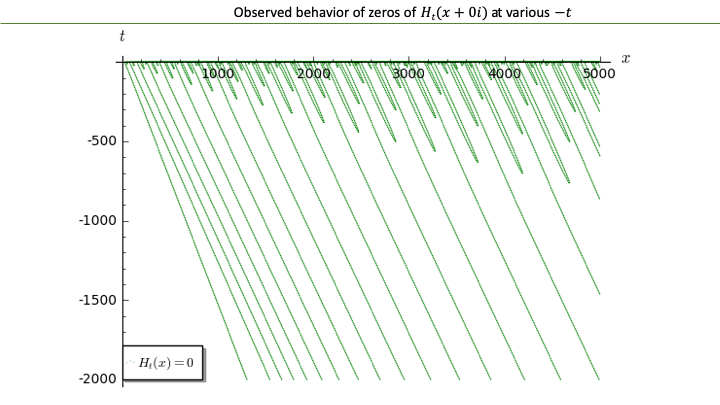
\includegraphics[width=0.8\linewidth]{traj_realzeros.png}
  \caption{Trajectories of real zeros up to $x=5000$. A clear pattern emerges when $x$ increases and $t$ becomes more negative.}
  \label{fig:realzeros}
\end{figure}

 \begin{figure}[h!]
  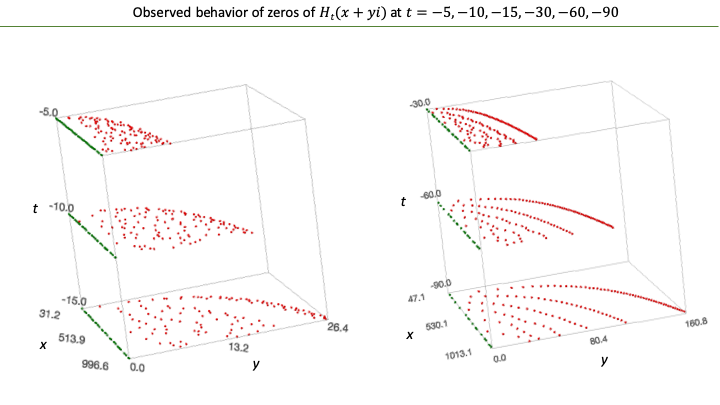
\includegraphics[width=0.8\linewidth]{traj_complexzeros.png}
  \caption{Trajectories of complex zeros at various negative values of $t$ up to $x=1000$. The complex zeros appear to organise themselves on curves when $x$ increases and $t$ becomes increasingly negative.}
  \label{fig:complexzeros}
\end{figure}


It is convenient to introduce the following coordinates: the shifted real argument
\begin{equation}\label{tx-def}
\tilde x \coloneqq x + \frac{\pi t}{4},
\end{equation}
a normalised version
\begin{equation}\label{n-def}
N \coloneqq \sqrt{\frac{\tilde x}{4\pi}} = \sqrt{\frac{x}{4\pi} + \frac{t}{16}}
\end{equation}
of that coordinate, and a further coordinate
$$ w \coloneqq \frac{t^2}{64\pi^2 N^3}.$$
For future reference we observe that
\begin{equation}\label{tx-form}
\tilde x = 4\pi N^2
\end{equation}
and (for negative values of $t$)
\begin{equation}\label{t-form}
t = - 8 \pi N^{3/2} w^{1/2}.
\end{equation}


\begin{claim}[Numerically observed phenomena]\label{nup}  
\begin{itemize}
\item[(i)]  For each natural number $n$, some of the complex zeroes of $H_t(x+iy)$ concentrate on the curve
\begin{equation}\label{yan}
 y = |t| \log \frac{N}{\sqrt{n(n+1)}} - 1.
\end{equation}
\item[(ii)]  For large values of $w$, the real zeroes of $H_t(x+iy)$ occur when $N$ is close to a half-integer.
\item[(iii)]  For medium values of $w$, the real zeroes of $H_t(x+iy)$ are confined to the region
$$ (\frac{9w}{4})^{1/3} - w < \{ 2N + \frac{1}{2}\} < 1-w $$
and occur when
$$ \frac{4 \sqrt{N}}{3} (1 - \{ 2N + \frac{1}{2}\} - w)^{3/2} + \frac{1}{4} $$
is close to an integer.
\end{itemize}
\end{claim}



\section{Heuristic approximations}

We now make some heuristic approximations to \eqref{11} in the regime $t<0$, $y \geq 0$, and $x \gg 1$, with $y$ not too large compared with $x$ (later on we will refine the approximation in certain subregimes).

From the functional equation for $H_t(x+iy) = H_t(-x-iy)$,  we have
$$H_t(x+iy) = \int_{\R} \frac{1}{8} \xi(\frac{1-ix+y}{2} - i |t|^{1/2} v) \frac{1}{\sqrt{\pi}} e^{-v^2}\ dv.$$
To cancel off an exponential decay factor in the $\xi$ function, it is convenient to shift the $v$ variable by $\pi |t|^{1/2}/8$, thus
\begin{align*}
H_t(x+iy) &= \frac{1}{8\sqrt{\pi}} \int_{\R} \xi(\frac{1-ix+y}{2} - i |t|^{1/2} v + \pi i |t|/8) e^{-(v - \pi |t|^{1/2}/8)^2}\ dv \\
&= \frac{\exp( \pi^2 t / 64)}{8\sqrt{\pi}} \int_{\R} \xi(\frac{1+y}{2}-\frac{i\tilde x}{2} - i |t|^{1/2} v) e^{-v^2 + \pi |t|^{1/2} v / 4}\ dv 
\end{align*}
where $\tilde x$ was defined by \eqref{tx-def}.  Next, from the definition of $\xi$ and the Stirling approximation we have
$$\frac{1}{8} \xi(s) \approx M_0(s) \zeta(s)$$
where
$$ M_0(s) \coloneqq \frac{1}{8} \frac{s(s-1)}{2} \pi^{-s/2} \sqrt{2\pi} \exp\left(\left(\frac{s}{2}-\frac{1}{2}\right) \Log \frac{s}{2} - \frac{s}{2}\right)$$
where $\Log$ denotes the standard branch of the complex logarithm.  Thus
$$H_t(x+iy) \approx \frac{\exp( \pi^2 t / 64)}{\sqrt{\pi}} \int_{\R} M_0(\frac{1+y}{2}-\frac{i\tilde x}{2} - i |t|^{1/2} v) \zeta(\frac{1+y}{2}-\frac{i\tilde x}{2} - i |t|^{1/2} v) e^{-v^2 + \pi |t|^{1/2} v / 4}\ dv.$$
By Taylor expansion we have
$$ M_0(\frac{1+y}{2}-\frac{i\tilde x}{2} - i |t|^{1/2} v) \approx M_0(\frac{1+y}{2}-\frac{i\tilde x}{2}) \exp( -\alpha( \frac{1+y}{2}-\frac{i\tilde x}{2} ) i |t|^{1/2} v + \alpha'(\frac{1+y}{2}-\frac{i\tilde x}{2}) \frac{-|t| v^2}{2} )$$
where 
$$\alpha(s) := \frac{M'_0(s)}{M_0(s)} = \frac{1}{2s} + \frac{1}{s-1} + \frac{1}{2} \Log \frac{s}{2\pi}$$
is the logarithmic derivative of $M_0$.  Assuming that $y$ is small compared to $\tilde x$, we have the approximations
$$
\alpha(\frac{1+y}{2}-\frac{i\tilde x}{2} ) \approx \frac{1}{2} \log \frac{\tilde x}{4\pi} - \frac{i\pi}{4}$$
and
$$ \alpha'(\frac{1+y}{2}-\frac{i\tilde x}{2} ) \approx \frac{i}{\tilde x}.$$
Using \eqref{tx-def}, we thus have
$$H_t(x+iy) \approx \frac{\exp( \pi^2 t / 64)}{\sqrt{\pi}} M_0(\frac{1+y}{2}-2\pi i N^2) \int_\R \exp(- i |t|^{1/2} v \log N - \frac{\pi |t|^{1/2} v}{4} - \frac{i |t| v^2}{8\pi N^2}) \zeta(\frac{1+y}{2}-2\pi i N^2 - i |t|^{1/2} v) e^{-v^2 + \frac{\pi |t|^{1/2} v}{4}}\ dv.$$
The two factors of $\exp( \frac{\pi |t|^{1/2} v}{4} )$ cancel.  In practice, the $\exp(-\frac{i|t|v^2}{8\pi N^2})$ term has proven to be fairly negligible, so we drop it to conclude that
$$ H_t(x+iy) \approx \frac{\exp( \pi^2 t / 64)}{\sqrt{\pi}} M_0(\frac{1+y}{2}-2\pi i N^2) \int_\R \exp( -i |t|^{1/2} v \log N ) \zeta(\frac{1+y}{2}-2\pi i N^2 - i |t|^{1/2} v) e^{-v^2}\ dv.$$
If we formally write $\zeta(s) = \sum_{n=1}^\infty \frac{1}{n^s}$ (ignoring convergence issues), we obtain
$$
 H_t(x+iy) \approx \frac{\exp( \pi^2 t / 64)}{\sqrt{\pi}} M_0(\frac{1+y}{2}-2\pi i N^2) \sum_{n=1}^\infty \int_\R \exp( -i |t|^{1/2} v \log N ) n^{-\frac{1+y}{2}+2\pi i N^2 + i |t|^{1/2} v} e^{-v^2}\ dv.
$$
We therefore expect zeroes $H_t(x+iy)$ to obey the approximate equation
$$\sum_{n=1}^\infty \int_\R \exp( -i |t|^{1/2} v \log\frac{N}{n} ) n^{-\frac{1+y}{2}+2\pi i N^2} e^{-v^2}\ dv.
\approx 0.$$
Evaluating the gaussian integral, we arrive at
\begin{equation}\label{fany}
 \sum_{n=1}^\infty f_n(N,y,t) \approx 0 
\end{equation}
where
\begin{equation}\label{fn-def}
 f_n(N,y,t) \coloneqq \exp( -\frac{|t|}{4} \log^2 \frac{N}{n} ) n^{-\frac{1+y}{2}+2\pi i N^2}.
\end{equation}

We now focus on two subregimes: one in which $|t|$ is small compared with $\tilde x$, and the other where $y=0$.

\subsection{Small $|t|$} 

The magnitude of $f_n(N,y,t)$ can be computed as
\begin{equation}\label{font}
 |f_n(N,y,t)| = \exp( \frac{1+y}{2} \log n -\frac{|t|}{4} \log^2 \frac{N}{n} ).
\end{equation}
The function $x \mapsto \frac{1+y}{2} \log x -\frac{|t|}{4} \log^2 \frac{N}{x}$ has first derivative
$$ \frac{1+y}{2x} - \frac{|t|}{2x} \log \frac{N}{x}$$
and is thus increasing in the region $y > |t| \log \frac{N}{x} - 1$ and decreasing outside of this region.  In particular, in the region
$$ |t| \log \frac{N}{n+1} - 1 < y < |t| \log \frac{N}{n}$$
for some fixed natural number $n$, we expect the terms $f_n, f_{n+1}$ to dominate the sum \eqref{fany}, so the zeroes of $H_t(x+iy)=0$ should be close to the zeroes of
$$ f_n(N,y,t) + f_{n+1}(N,y,t) = 0.$$
The latter of course lies on the curve $|f_n(N,y,t)| = |f_{n+1}(N,y,t)|$, which by \eqref{font} and some algebra may be simplified to
$$ y = |t| \log \frac{N}{\sqrt{n(n+1)}} - 1.$$
This supports Claim \ref{nup}(i).

{\bf add remark about how one can see finer oscillations in the zeroes by retaining a few more terms in \eqref{fany}.}

\subsection{Real zeroes}

Now we take $y=0$. 
We substitute \eqref{t-form} into \eqref{fn-def} and use the Taylor approximation $\log \frac{N}{n} \approx \frac{n-N}{N}$ to then obtain
$$ f_n(N,0,t) \approx  \exp( -2\pi N^{-1/2} w^{1/2} (n-N)^2  - \frac{1}{2} \log n + 2\pi i N^2 \log n).$$
The gaussian factor $\exp( -2\pi N^{-1/2} w^{1/2} (n-N)^2 )$ localises $n$ to $N$, and we then use the approximations
$$ \frac{1}{2} \log n \approx \frac{1}{2} \log N$$
and
$$ 2\pi i N^2\log n \approx 2\pi i N^2 (\log N + \frac{n-N}{N} - \frac{(n-N)^2}{2N^2} + \frac{(n-N)^3}{3N^3})$$
so \eqref{fany} then becomes (after canceling some terms independent of $n$)
$$ \sum_{n=1}^\infty \exp( -2\pi N^{-1/2} w^{1/2} (n-N)^2  + 2\pi i N (n-N) - \pi i (n-N)^2 + \frac{2\pi i}{3N} (n-N)^3 ) \approx 0.$$
We compute
\begin{align*}
\exp( 2\pi i N(n-N) - \pi i (n-N)^2 ) &= \exp( -\pi i n^2 + 4\pi i N n - 3 \pi i N^2 ) \\
&= \exp( \pi i n + 4\pi i N n - 3 \pi i N^2 ) \\
&= \exp(2\pi i \{ 2N + \frac{1}{2} \} n - 3 \pi i N^2 )
\end{align*}
where $\{x\}$ denotes the fractional part of $x$.  The above equation thus becomes
$$
 \sum_{n=1}^\infty \exp( -2\pi N^{-1/2} w^{1/2} (n-N)^2 + 2\pi i n \{2N + \frac{1}{2}\} + \frac{2\pi i}{3N} (n-N)^3) \approx 0.$$
In view of the gaussian factor, we now allow $n$ to range over the integers rather than the natural numbers.  Using Poisson summation, we arrive at
$$ \sum_m g_m(N,w) \approx 0$$
where
$$g_m(N,w) \coloneqq \int_\R \exp( -2\pi N^{-1/2} w^{1/2} (X-N)^2 - 2\pi i X (m - \{2N + \frac{1}{2}\}) + \frac{2\pi i}{3N} (X-N)^3)\ dX.$$
We can shift $X$ by $N$ to obtain
$$ g_m(N,w) = e^{-2\pi i N (m - \{2N + \frac{1}{2}\})} \int_\R \exp( -2\pi N^{-1/2} w^{1/2} X^2- 2\pi i X (m - \{2N + \frac{1}{2}\}) + \frac{2\pi i}{3N} X^3)\ dX.$$

Suppose we neglect the third order term $\frac{2\pi i}{3N} X^3$.  Then 
\begin{align}
 g_m(N,w) &\approx e^{2\pi i N (m - \{2N + \frac{1}{2}\})} \int_{\bf R} \exp( -2\pi N^{-1/2} w^{1/2} X^2 - 2\pi i X (m - \{2N + \frac{1}{2}\})\ dX \nonumber\\
&\approx \sqrt{\frac{N^{1/2}}{2w^{1/2}}} e^{-2\pi i N (m - \{2N + \frac{1}{2}\})} \exp( -\frac{(m - \{2N + \frac{1}{2}\})^2 N^{1/2}}{4w^{1/2}} ).\label{one}
\end{align}
This decays quickly for $m$ far from $\{2N + \frac{1}{2}\}$, so we expect the $m=0$ and $m=1$ terms to dominate, thus we arrive at
\begin{equation}\label{simple}
 g_0(N,w) + g_1(N,w) \approx 0.
\end{equation}
Inserting the approximation \eqref{one}, and cancelling common terms, we arrive at
$$ 
1 + e^{-2\pi i N} \exp( -\frac{( 1 - 2\{2N + \frac{1}{2}\}) N^{1/2}}{4 w^{1/2}} ) \approx 0.$$
This has solutions when $N$ is a half-integer.
This supports Claim \ref{nup}(ii).

Now we look at smaller values of $w$.  Here we do not omit the $\frac{2\pi i}{3N} X^3$ term, but continue to use the simplified equation \eqref{simple}. We may write
$$
g_m(N,w) = \exp(-i N c_m ) \int_\R \exp( \frac{ia}{3} X^3 - i b X^2 - i c_m X )\ dX$$
where
\begin{align*}
a &\coloneqq \frac{2\pi}{N} \\
b &\coloneqq -2 \pi i N^{-1/2} w^{1/2} \\
c_m &\coloneqq 2 \pi (m - \{ 2N + \frac{1}{2} \} ).
\end{align*}
If we make the change of variables $X = a^{-1/3} (t + ba^{-2/3})$ and formally shift the contour of integration, we obtain
$$ g_m(N,w) = a^{-1/3} \exp( -i N c_m - 2 i b^3 a^{-2}/3 - i bc_m a^{-1}) \int_\R \exp( \frac{it^3}{3} - i(c_m a^{-1/3} + b^2 a^{-4/3}) t )\ dt.$$
Since the Airy function $\mathrm{Ai}$ is given by the formula
\begin{align*}
\mathrm{Ai}(x) &= \frac{1}{\pi} \int_0^\infty \cos(\frac{t^3}{3} + xt)\ dt \\
&= \frac{1}{2\pi} \int_{\bf R} \exp(i\frac{t^3}{3} + ixt)\ dt
\end{align*}
we conclude that
$$ g_m(N,w) = 2\pi a^{-1/3} \exp( -i N c_m - 2 i b^3 a^{-2}/3 - i bc_m a^{-1}) \mathrm{Ai}( - (c_m a^{-1/3} + b^2 a^{-4/3}) ).$$
Inserting this into \eqref{simple}, we arrive at
$$ \mathrm{Ai}( - (c_0 a^{-1/3} + b^2 a^{-4/3}) ) + \exp(- 2\pi iN - 2\pi ib a^{-1} ) \mathrm{Ai}( - (c_0 a^{-1/3} + b^2 a^{-4/3} + 2\pi a^{-1/3}) ) ) \approx 0.$$

Substituting the definitions of $a,b,c_0$,we obtain
\begin{equation}\label{non}
 \mathrm{Ai}( (2\pi)^{2/3} N^{1/3} ( \{ 2N + \frac{1}{2}\} + w ) ) + \exp( -2\pi i N - 2 \pi N^{1/2} w^{1/2}  )
\mathrm{Ai}( (2\pi)^{2/3} N^{1/3} ( \{ 2N + \frac{1}{2}\} + w - 1) ) \approx 0.
\end{equation}
The Airy function oscillates for negative reals and is positive for positive reals.  We then expect the zeroes of the above equation to be located in the region where
$$ \{ 2N + \frac{1}{2}\} + w - 1 < 0$$
and in which the amplitude of the second term dominates that of the first term. Up to polynomial factors, $\mathrm{Ai}(x)$ behaves like $e^{-\frac{2}{3x^{3/2}}}$ for positive $x$ and oscillates with bounded amplitude for negative $x$, thus we expect
$$ \exp( -\frac{2}{3} [ (2\pi)^{2/3} N^{1/3} ( \{ 2N + \frac{1}{2}\} + w ) ]^{3/2} ) \leq
\exp( -2 \pi N^{1/2} w^{1/2} )$$
which after some algebra simplifies to
$$ \{ 2N + \frac{1}{2} \} + w - (\frac{9w}{4})^{1/3} > 0.$$
In this region, the second term in \eqref{non} dominates, leading us to
$$ \mathrm{Ai}( (2\pi)^{2/3} N^{1/3} ( \{ 2N + \frac{1}{2}\} + w - 1) ) \approx 0.$$
The zeroes of $\mathrm{Ai}(x)=0$ occur when $\frac{2}{3} (-x)^{3/2} + \frac{\pi}{4}$ is close to a multiple of $\pi$, so we arrive at
$$ \frac{2}{3} 2 \pi N^{1/2} (1 - \{ 2N + \frac{1}{2}\} - w)^{3/2} + \frac{\pi}{4} \approx 0 \hbox{ mod } \pi $$
or equivalently
$$ \frac{4 \sqrt{N}}{3} (1 - \{ 2N + \frac{1}{2}\} - w)^{3/2} + \frac{1}{4} \approx 0 \hbox{ mod } 1 .$$
This supports Claim \ref{nup}(iii).


\begin{remark}  The above analysis also allows one to predict how many zeroes one would expect to participate in the patterns observed in Claim \ref{nup}.  In the region $0 \leq x \leq x_*$, the Riemann-von Mangoldt formula for $H_t$ (see \cite[Theorem 4.2]{brad}) shows that the number of zeroes of $H_t(x+iy)=0$ is approximately
$$ \frac{x_*}{4\pi} \log \frac{x_*}{4\pi} - \frac{x_*}{4\pi} \approx N_*^2 \log N_*^2 $$
where $N_* := \frac{x_*}{4\pi}$.  On the other hand, by inspecting the variation in phase of $f_{n+1}(N,y,t)/f_n(N,y,t)$, we expect the number of such zeroes lying near the curve \eqref{yan} with $0 \leq x \leq x_*$ to be roughly $N_*^2 \log \frac{n+1}{n}$ for a fixed choice of $t$.  The number of zeroes obeying Claim \ref{nup}(ii) should be approximately $N_*$, while the number obeying Claim \ref{nup}(ii) is $O( N_*^{3/2})$.  In particular only a small minority of the zeroes should remain real as $t$ becomes negative.
\end{remark}



\begin{thebibliography}{99} 

%\bibitem{arias}
%J. Arias de Reyna, \emph{High-precision computation of Riemann's zeta function by the Riemann-Siegel asymptotic formula, I}, Mathematics of Computation, \textbf{80} (2011), 995--1009.
%
%\bibitem{arias-lune}
%J. Arias de Reyna, J. Van de lune, \emph{On the exact location of the non-trivial zeroes of Riemann's zeta function}, Acta Arith. \textbf{163} (2014), 215--245.
%
%\bibitem{boyd}
%W. G. C. Boyd, \emph{Gamma Function Asymptotics by an Extension of the Method of Steepest Descents}, Proceedings: Mathematical and Physical Sciences, Vol. 447, No. 1931 (Dec. 8, 1994), 609--630.

\bibitem{debr}
N. C. de Bruijn, \emph{The roots of trigonometric integrals}, Duke J. Math. \textbf{17} (1950), 197--226.

%\bibitem{cmmrs}
%A. Chang, D. Mehrle, S. J. Miller, T. Reiter, J. Stahl, D. Yott, \emph{Newman's conjecture in function fields}, J. Numb. Thy. \textbf{157} (2015), 154--169.
%

\bibitem{cnv}
G. Csordas, T. S. Norfolk, R. S. Varga, \emph{A lower bound for the de Bruijn-Newman constant $\Lambda$}, Numer. Math. \textbf{52} (1988), 483--497.

\bibitem{cosv}
G. Csordas, A. M. Odlyzko, W. Smith, R. S. Varga, \emph{A new Lehmer pair of zeros and a new lower bound for the De Bruijn-Newman constant Lambda}, Electronic Transactions on Numerical Analysis. \textbf{1} (1993), 104--111.

\bibitem{crv}
G. Csordas, A. Ruttan, R.S. Varga, \emph{The Laguerre inequalities with applications
to a problem associated with the Riemann hypothesis}, Numer. Algorithms, \textbf{1} (1991), 305--329.

\bibitem{csv}
G. Csordas, W. Smith, R. S. Varga, \emph{Lehmer pairs of zeros, the de Bruijn-Newman constant $\Lambda$, and the Riemann hypothesis},  Constr. Approx. \textbf{10} (1994), no. 1, 107--129. 

\bibitem{kkl}
H. Ki, Y. O. Kim, and J. Lee, \emph{On the de Bruijn-Newman constant}, Advances in Mathematics, \textbf{22} (2009), 281--306.

%\bibitem{lehmer}
%D. H. Lehmer, \emph{On the roots of the Riemann zeta-function}, Acta Math. \textbf{95} (1956), 291--298.

%\bibitem{montgomery}
%H. L. Montgomer
%y, \emph{The pair correlation of zeros of the zeta function}, Analytic number theory (Proc. Sympos. Pure Math., Vol. XXIV, St. Louis Univ., St. Louis, Mo., 1972), 181--193. Amer. Math. Soc., Providence, R.I., 1973.
%
%\bibitem{MoVa}
%H. L. Montgomery, R. C. Vaughan, Multiplicative number theory. I. Classical theory. Cambridge Studies in Advanced Mathematics, 97. Cambridge University Press, Cambridge, 2007.

\bibitem{newman}
C. M. Newman, \emph{Fourier transforms with only real zeroes}, Proc. Amer. Math. Soc. \textbf{61} (1976), 246--251.

\bibitem{nrv}
T. S. Norfolk, A. Ruttan, R. S. Varga, \emph{A lower bound for the de Bruijn-Newman
constant $\Lambda$ II.}, in A. A. Gonchar and E. B. Saff, editors, Progress in Approximation
Theory, 403--418. Springer-Verlag, 1992.

\bibitem{odlyzko}
A. M. Odlyzko, \emph{An improved bound for the de Bruijn-Newman constant}, Numerical Algorithms \textbf{25} (2000), 293--303.

%\bibitem{euler}
%T. K. Petersen, Eulerian numbers.  With a foreword by Richard Stanley. Birkh\"auser Advanced Texts: Basler Lehrb\"ucher. Birkh\"auser/Springer, New York, 2015.
%
%\bibitem{platt}
%D. J. Platt, \emph{Isolating some non-trivial zeros of zeta}, Math. Comp. 86 (2017), 2449--2467.
%
\bibitem{polya}
G. Polya, {\"Uber trigonometrische Integrale mit nur reelen Nullstellen}, J. Reine Angew. Math. \textbf{58} (1927), 6--18. 

\bibitem{polymath15}
D. H. J. Polymath, \emph{Effective approximation of heat flow evolution of the Riemann $\xi$ function, and an upper bound for the de Bruijn-Newman constant}, preprint.

\bibitem{github}
D. H. J. Polymath, {\tt github.com/km-git-acc/dbn\_upper\_bound}

\bibitem{brad}
B. Rodgers, T. Tao, \emph{The De Bruijn-Newman constant is nonnegative}, preprint. {\tt arXiv:1801.05914}

\bibitem{saouter}
Y. Saouter, X. Gourdon, P. Demichel, \emph{An improved lower bound for the de Bruijn-Newman constant}, Mathematics of Computation. \textbf{80} (2011), 2281--2287. 

%\bibitem{stopple}
%J. Stopple, \emph{Notes on Low discriminants and the generalized Newman conjecture}, Funct. Approx. Comment.
%Math., vol. 51, no. 1 (2014), 23--41.
%
%\bibitem{stopple-2}
%J. Stopple, \emph{Lehmer pairs revisited}, Exp. Math. \textbf{26} (2017), no. 1, 45--53. 

\bibitem{tr}
H. J. J. te Riele, \emph{A new lower bound for the de Bruijn-Newman constant}, Numer. Math., \textbf{58} (1991), 661--667.

\bibitem{titch}
E. C. Titchmarsh, The Theory of the Riemann Zeta-function, Second ed. (revised by D. R. Heath-Brown), Oxford University Press, Oxford, 1986.	


\end{thebibliography} 
























\end{document}
